\documentclass[a4paper, 12pt]{article}
\usepackage[utf8]{inputenc}
\usepackage[T1]{fontenc}
\usepackage{times}
\usepackage[spanish]{babel}
% \usepackage{hyperref} % Paquete para hipervínculos
\usepackage[left=2.5cm, right=2.5cm, top=2.5cm, bottom=2.5cm]{geometry}
\linespread{1.5}
\usepackage{graphicx} % Required for inserting images
\usepackage{amsmath}
\usepackage{titlesec} % Paquete para el formato de los títulos
\usepackage{hyperref}

\hypersetup{
	colorlinks=true,
	urlcolor=blue,
	linkcolor=black  % Cambia el color de los índices a azul oscuro
}

\setlength{\parindent}{0pt}

% Reducir el espacio entre los apartados del índice
\makeatletter
\renewcommand*\l@section{\@dottedtocline{1}{0em}{1.5em}}
\renewcommand*\l@subsection{\@dottedtocline{2}{1.5em}{2.5em}}
\renewcommand*\l@subsubsection{\@dottedtocline{3}{4.0em}{3.5em}}
\makeatother

\begin{document}
%-------------------------------------------------------
% PORTADA
%-------------------------------------------------------
\begin{titlepage}
	\begin{center}
		
\includegraphics[scale=0.9]{images.png}
		\vspace{1.75cm}
		
		\large
		\textbf{ESCUELA TÉCNICA SUPERIOR DE INGENIERÍA INFORMÁTICA}
		\vspace{1cm}
		
		\large
		\textbf{GRADO EN INGENIERÍA INFORMÁTICA}
		
		
		
		\large
		\textbf{Curso Académico 2023/2024}
		
		\vspace{1cm}
		\large
		\textbf{Práctica 1}
		
		\vspace{2cm}
		
		\large
		\textbf{DETECCIÓN DE SEÑALES VIALES}
		
		\vspace{2cm}
		
		\large
		Cristian Fernando Calva Troya \\
		Luis Ovejero Martín \\
		Jaime Rueda Carpintero
		\vspace{1cm}
	\end{center}
\end{titlepage}

\newpage
\thispagestyle{empty} 
\mbox{} 

\newpage
%-------------------------------------------------------
% Tabla de figuras
%-------------------------------------------------------
\newpage
\listoffigures
\newpage

%-------------------------------------------------------
% Tabla de contenidos
%-------------------------------------------------------
{\small
	\tableofcontents 
}
\newpage

%-------------------------------------------------------
% 1. Introducción
%-------------------------------------------------------
\section{Introducción}
En esta práctica, abordamos el desafío de la detección de señales viales utilizando técnicas de procesamiento de imágenes. Nuestro objetivo es desarrollar un sistema capaz de identificar y localizar paneles de tráfico en imágenes capturadas por vehículos en carretera.

Para lograrlo, aplicamos una variedad de técnicas de procesamiento de imágenes, desde la normalización y filtrado de color, hasta la detección de regiones de interés y la correlación por máscaras. Estas técnicas nos permiten preprocesar las imágenes de manera adecuada para extraer las características relevantes y luego identificar los paneles de señalización de tráfico en base a un panel ideal.


%-------------------------------------------------------
% 2. OBJETIVOS Y METODOLOGIAS
%-------------------------------------------------------
\section{Objetivos y metodología}

\subsection{Descripción del problema y objetivos}
Se desea construir un sistema para la detección automática de paneles informativos de tráfico de color azul, en imágenes realistas que han sido tomadas desde un coche. Los paneles se han diseñado para que sean fácilmente distinguibles del entorno en cualquier condición de luz, color de fondo y climatología.

El objetivo de esta práctica es crear una aplicación que recibiendo una lista de imágenes sea capaz de determinar si hay o no paneles informativos de tráfico y en caso de haberlos determinar en que región de la imagen se encuentran. 

\subsection{Tecnologías}
Para el desarrollo de esta práctica hemos usado el lenguaje \textit{Python} y, principalmente la librería de \textit{OpenCV} (\textit{cv2}), entre otras como, \textit{matplotlib}, \textit{numpy}, \textit{os} y \textit{math}. 

El código de la practica ha sido desarrollado en \textit{jupiter notebook}.

%-------------------------------------------------------
% 3. DESCRIPCIÓN INFORMATICA
%-------------------------------------------------------

\section{Creación de la aplicación}
\subsection{Normalización}
Una misma imagen tomada en el mismo lugar variará en función de diversos factores como puede ser la luz, climatología, orientación de la cámara y otros muchos factores. En nuestro caso, el mayor problema con el que nos encontramos es con la niebla y los paneles rotados. Al haber nieble en la escena es posible que nos encontremos con una imagen mucha menos nítida y menos saturada. En cuanto a la orientación al tener un cuadrado recto de la detección que no podemos rotar, es posible que tengamos problemas para posicionarlo. A continuación se explicarán los métodos usados para evitar este ruido adverso.
\subsubsection{Corrección de color}
Uno de los problemas con los que se puede enfrentar el detector es la iluminación de la escena, en concreto con la iluminación producida por la niebla. Cuando hay niebla se pierde nitidez y saturación en la escena. Objetos que se encuentran un tanto alejados desde la posición desde donde tomamos las fotos van a visualizarse de forma borrosa y sin mucha claridad. Este es un problema para el detector ya que para las imagénes donde aparecía niebla el detector no era capaz de detectar ningún panel.
Para ello, aplicamos la siguiente fórmula sencilla para obtener la saturación para un imagen:
	\begin{equation}
		S = \frac{\sum_{i=0}^p s(i)}{p}
	\end{equation}
Donde:
\begin{itemize}
    \item $S$ = índice de saturación de la imagen
    \item $p$ = número de píxeles totales de la imagen
    \item $s$ = saturación del píxel i
\end{itemize}
Para obtener la saturación de cada píxel, la imagen es transformada al formato HSV. Este formato tiene tres componentes distintas: matiz, saturación y valor. En nuestro caso tendremoss en cuenta la saturación ya que es la componente que más diferencia hay entre una imagen normal y una con niebla.

Después de obtener esta media de saturación para cada imagen, establecemos un umbral, donde si una imagen no supera ese umbral entonces tendremos que aplicarle un filtro de aumento de saturación. Después de ejecutar este algoritmo observamos que la mayoría de imágenes con niebla no eran capaces de superar el umbral de 27, por lo que ese umbral es el establecido. Las demás imágenes sin niebla no pasarán por este filtro. El filtro en cuestión consiste en tomar la saturación de los píxeles y multiplicarlos por 3, para obtener así una imagen mucho más saturada. Así quedaría el proceso de normalización del color, pasando una imagen con niebla a una mucho más saturada, como podemos ver en la \textbf{\hyperref[fig:saturada]{Fig. 1}}.

\begin{figure}[h]
	\centering
	\caption{Imagen con niebla saturada}\vspace{0.5cm}
	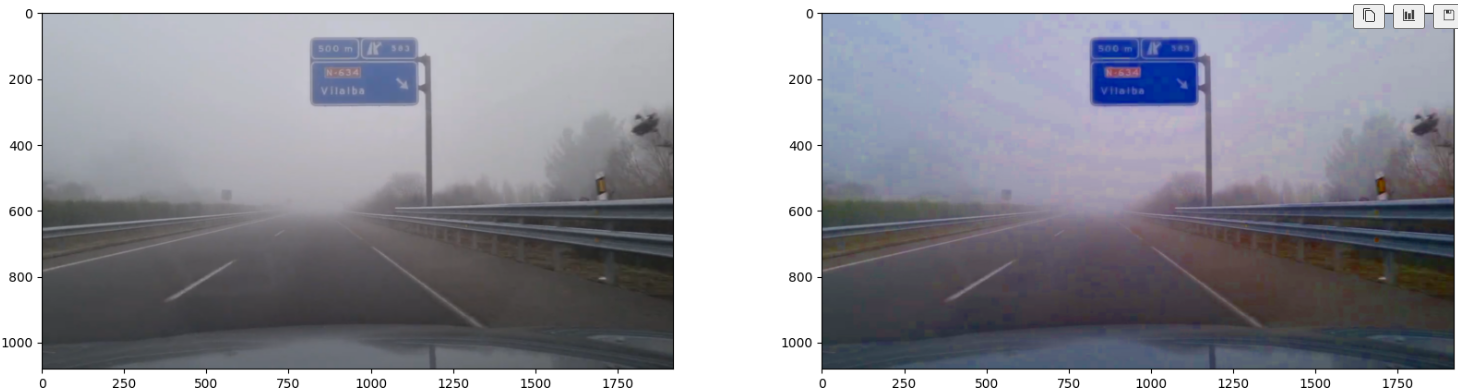
\includegraphics[width=0.8\linewidth]{img/saturated_img.png}
	\label{fig:saturada}
\end{figure}

\subsubsection{Corrección de ángulo}
\begin{figure}[h]
	\centering
	\caption{Corrección de angulo de la imagen}\vspace{0.5cm}
	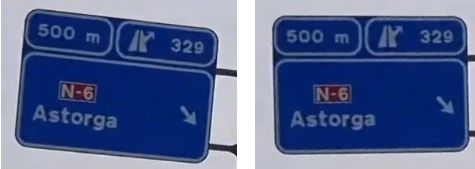
\includegraphics[width=0.8\linewidth]{img/norma_angulo}
	\label{fig:normaangulo}
\end{figure}

Otro de los problemas presentes a la hora de procesar las imágenes, para su detección, es la posición de los objetos a detectar. En ocasiones, ya sea por el ángulo de la cámara o la misma posición del cartel respeto a nosotros, puede ocurrir un cierto desfase en el angulo deseado. En la \textbf{\hyperref[fig:normaangulo]{Fig. 2}} podemos observar un pequeño ejemplo del problema inicial y el resultado deseado, que nos dará una mejor detección de las secciones. Para poder abarcar el problema hemos optado por realizar una corrección a la imagen completa. 

Los pasos a seguir para conseguir el angulo de desfase son los siguientes:



\begin{quote}
	\textbf{1.} Aplicamos una detección de color azul ya que respecto a las diferentes pruebas, ha dado mejores resultados para eliminar las zonas no deseadas y poder centrarnos en las secciones más azules (los paneles deseados.) En la \textbf{\hyperref[fig:imagebluef]{Fig. 3}} podemos ver un ejemplo de los posibles resultados.
	\begin{figure}[h]
		\centering
		\caption{Imagen tras aplicar filtro azul}\vspace{0.5cm}
		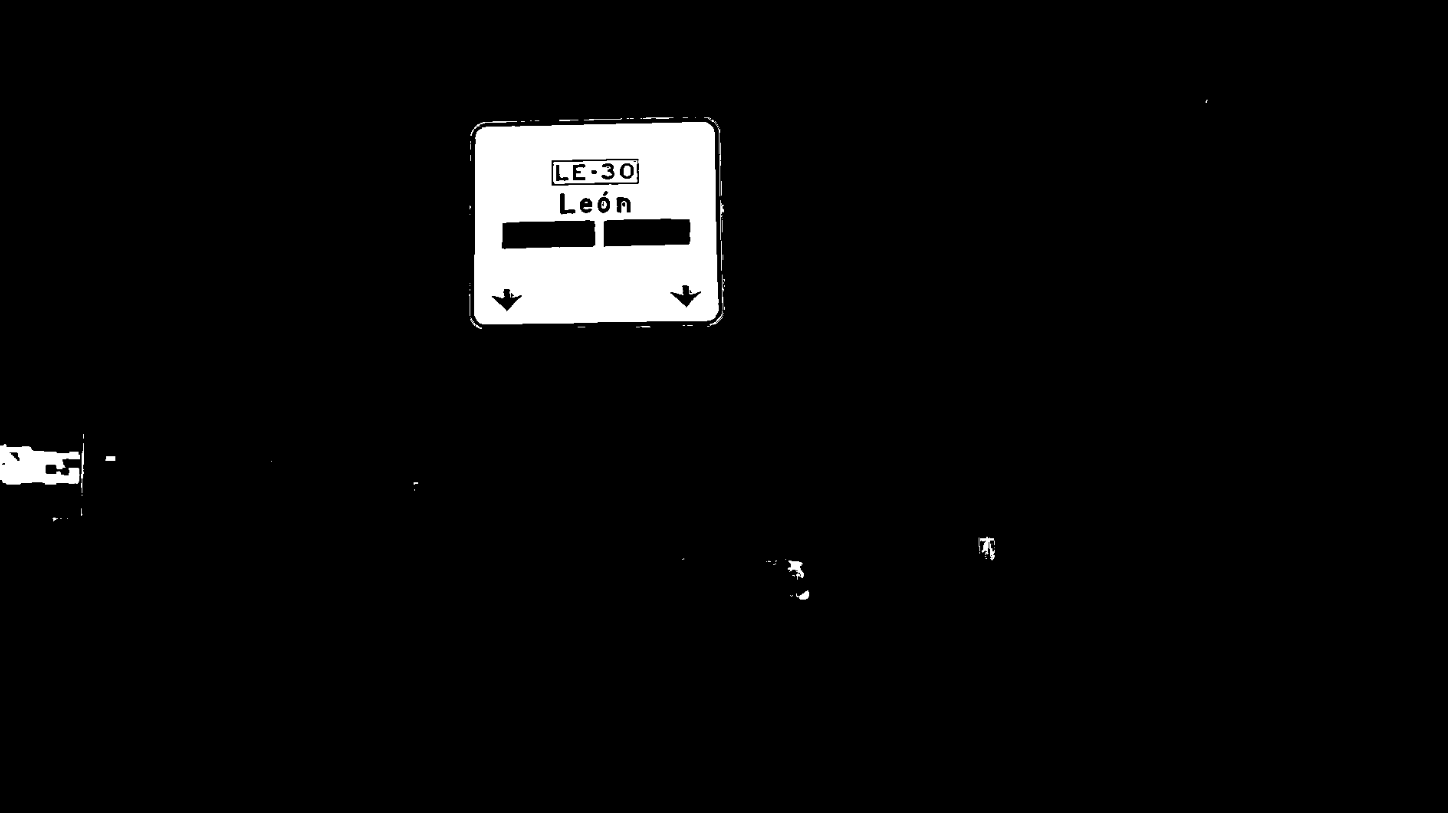
\includegraphics[width=0.6\linewidth]{img/image_blue_f}
		\label{fig:imagebluef}
	\end{figure}
	
	\textbf{2.} Realizamos una detección de bordes horizontales. Ya que haremos la corrección en función de como estén estos orientados. En la \textbf{\hyperref[fig:imageboderh]{Fig. 4}} se ve que conseguimos las secciones deseadas.
	
	\begin{figure}[h]
		\centering
		\caption{Imagen tras aplicar sobel}\vspace{0.5cm}
		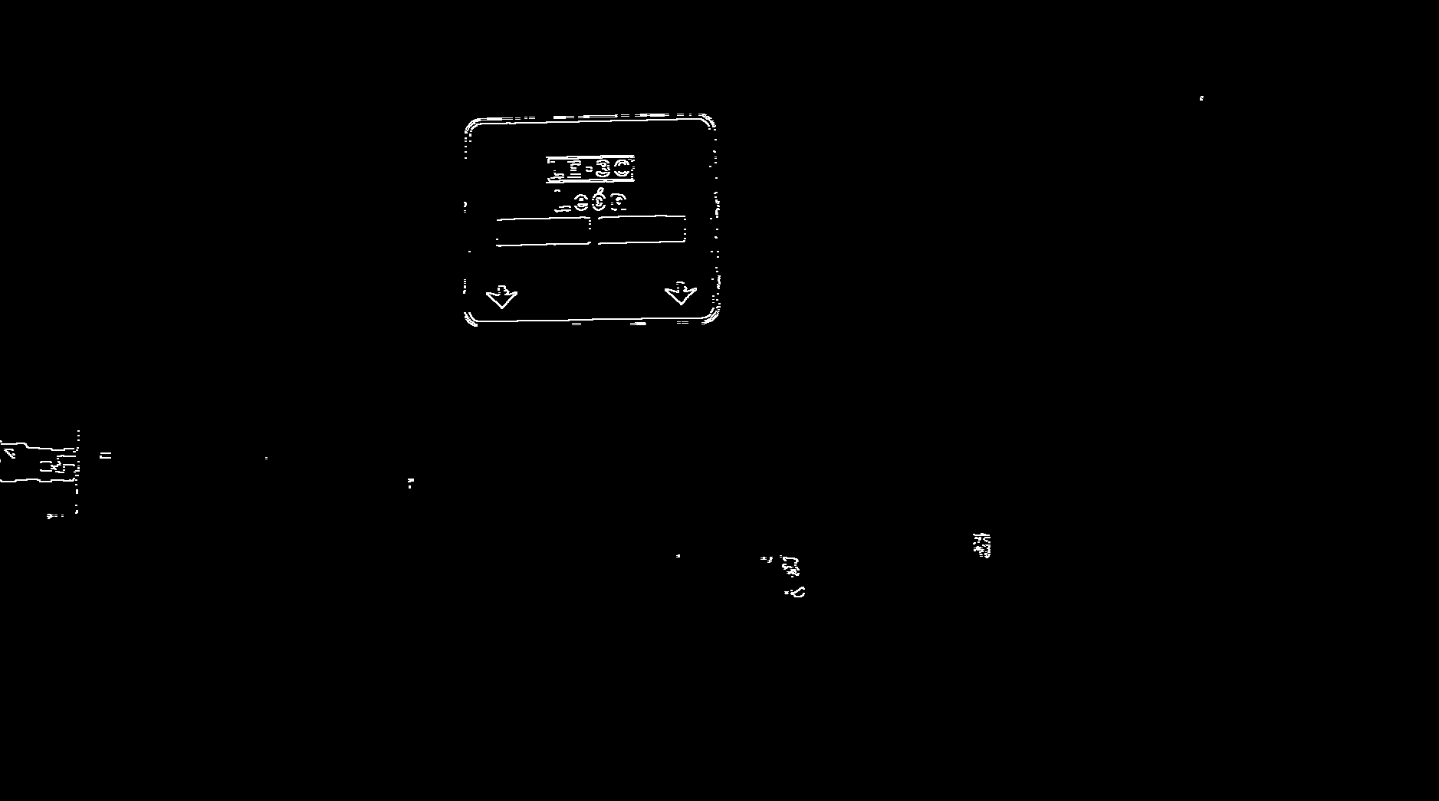
\includegraphics[width=0.6\linewidth]{img/image_boder_h}
		\label{fig:imageboderh}
	\end{figure}
	\textbf{3.} Finalmente con el algoritmo de Hough extraemos líneas presentes en la imagen, dando como resultado las rectas horizontales. En la \textbf{\hyperref[fig:imagewithlines]{Fig. 5}} se visualizan las rectas detectadas, y se calcula el angulo de cada uno de ellas haciendo uso de las coordenadas $(x, y)$ y $(x2, y2)$, de estas nos quedaremos con un desfase intermedio. Finalmente con el ángulo de cada imagen, corregimos el giro sobre la imagen original, tal y como se muestra en la \textbf{\hyperref[fig:00057co]{Fig. 6}}.
	
	\begin{figure}[h]
		\centering
		\caption{Imagen tras detectar lineas y ángulos de desfase}\vspace{0.5cm}
		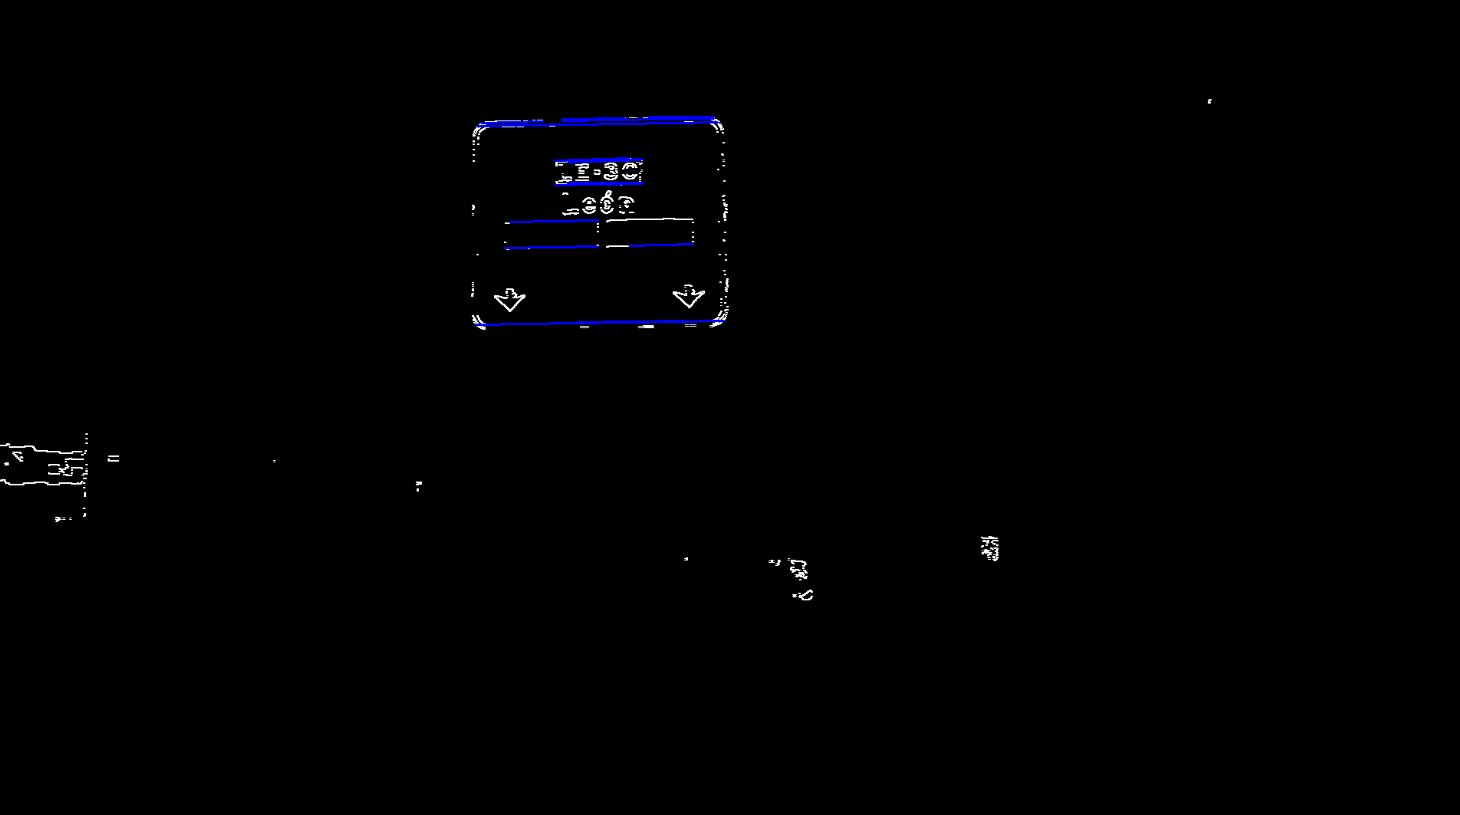
\includegraphics[width=0.6\linewidth]{img/image_with_lines+}
		\label{fig:imagewithlines}
	\end{figure}
	
	\begin{figure}[h]
		\centering
		\caption{Corrección de angulo de imagen}\vspace{0.5cm}
		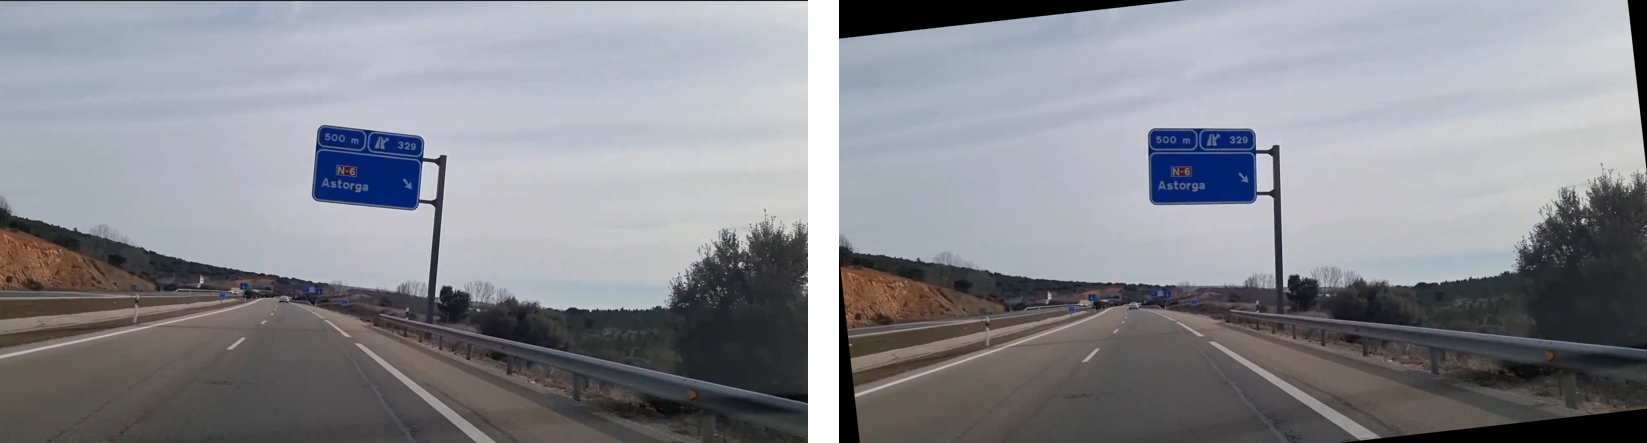
\includegraphics[width=0.7\linewidth]{img/00057_co}
		\label{fig:00057co}
	\end{figure}
	
\end{quote}

\subsection{Detección de regiones de alto contraste}
\subsubsection{Aplicar el filtro de azul}
Antes de empezar a detectar regiones, vamos a aplicar el filtro de azul sobre las imágenes normalizadas. Esto lo hacemos con la idea de mejorar la detección de los carteles, ya que al aplicar el filtro de azul podemos determinar de forma más eficaz la zona de imagen que puede pertenecer a un cartel. 

\subsubsection{MSER}
Una vez hemos aplicado este filtro a las imágenes ya podemos empezar a detectar regiones sobre las máscaras que hemos generado con el paso anterior.

Para detectar las regiones de alto contraste definimos la función \textit{mser}. Esta recibirá la lista de imágenes normalizadas y la lista de mascaras que hemos creado al aplicar el filtro de azul. 
Crearemos dos listas que nos servirán para guardar aquellas imágenes sobre las que vamos a dibujar las regiones que detectemos y la otra para guardar las regiones detectadas. 


La función va a iterar sobre la lista de imágenes y creará una copia de la imagen normalizada para dibujas las regiones y una copia de la máscara sobre la que aplicará \textit{MSER}. Antes de aplicar el algoritmo dilatamos la mascara y restamos la máscara original a la máscara dilatada para obtener una imagen de bordes. Tras esto creamos un \textit{MSER} y ajustamos los parámetros para filtrar un poco las regiones que pueda detectar, por ejemplo, haciendo que el área mínima de las regiones que detecte sea 900 y que la máxima sea 5000. 


Las regiones detectadas en una imagen se guardaran en la variable llamada \textit{polygons}. Sobre esa lista iteraremos a continuación y para cada elemento de la lista aplicaremos la función \textit{convexHull} de \textit{openCV}, con la finalidad de hallar el casco convexo de un conjunto de puntos. Esto quiere decir que la usaremos para determinar el perímetro de la región que hemos detectado. Guardaremos estos perímetros en la lista \textit{hulls}, que usaremos más adelante para poder dibujar las regiones en la imagen. También guardamos la lista de regiones detectadas en \textit{detected\_regions} y finalmente dibujaremos las regiones sobre la copia de la imagen y la guardaremos en la lista que hemos creado al principio para ello. Por último mostramos la primera y última imagen con las regiones dibujadas y devolvemos las listas de las imágenes con las regiones dibujadas y la lista de las regiones detectadas.

Tras ejecutar la función deberían aparecer las imágenes que podemos ver en la \textbf{\hyperref[fig:imagenesMSER]{Fig. 7}}

\begin{figure}[h]
	\centering
	\caption{Imagen tras aplicar MSER y dibujar las regiones detectadas}\vspace{0.5cm}
	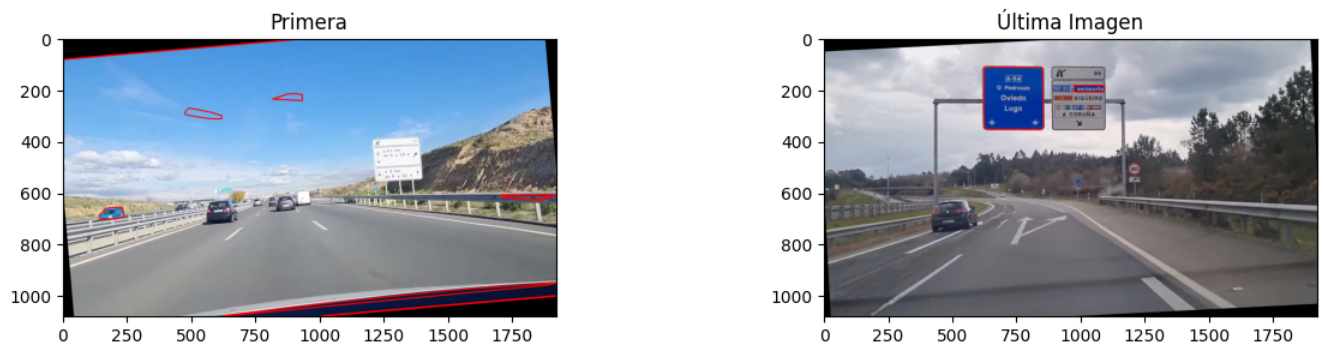
\includegraphics[width=0.6\linewidth]{img/ImagenesTrasMSER}
	\label{fig:imagenesMSER}
\end{figure}


En la siguiente celda del \textit{notebook} vemos un bloque de código con un bucle \textit{for} que está comentado, lo podemos descomentar y ejecutar para ver el resultado de nuestra función sobre el resto de imágenes de test. Para pasar las fotos simplemente vamos pulsando cualquier tecla. En caso de querer parar tenemos que pulsar el cuadrado de arriba a la izquierda y cerrar la ventana para terminar la ejecución. 


\subsubsection{Extraer los píxeles de la región en un rectángulo}
Para este paso vamos a definir la función \textit{rectangle\_of\_regions} que tiene como objetivo dibujar, usando \textit{cv2.boundingRect}, un rectángulo alrededor de las regiones detectadas en el paso anterior. La función recibirá la lista de imágenes normalizadas y la lista de las regiones detectadas en el paso anterior.
Se creará una lista en la que se añadirán las imágenes con los rectángulos dibujados. Iteraremos sobre las imágenes de test y crearemos una copia de cada imagen. Ahora iteraremos sobre las regiones de la imagen sobre la que estamos trabajando y usaremos \textit{cv2.boundingRect}, para obtener el punto superior izquierdo de la región y el ancho y alto de la misma y con ello dibujaremos el rectángulo con \textit{cv2.rectangle}. 


Tras dibujar las regiones añadimos la imagen a la lista, imprimimos la primera y la última de estas imágenes y devolvemos la lista donde las hemos guardado. 


Al igual que en la región anterior, tenemos una celda de código comentado que podremos usar para poder ver el resultado en el resto de imágenes.

Un ejemplo de los resultados que podemos ver en estas imágenes resultado lo vemos en la \textbf{\hyperref[fig:Rectangulos]{Fig. 8}}
\begin{figure}[h]
	\centering
	\caption{Imagen tras dibujar un rectángulo en cada región detectada}\vspace{0.5cm}
	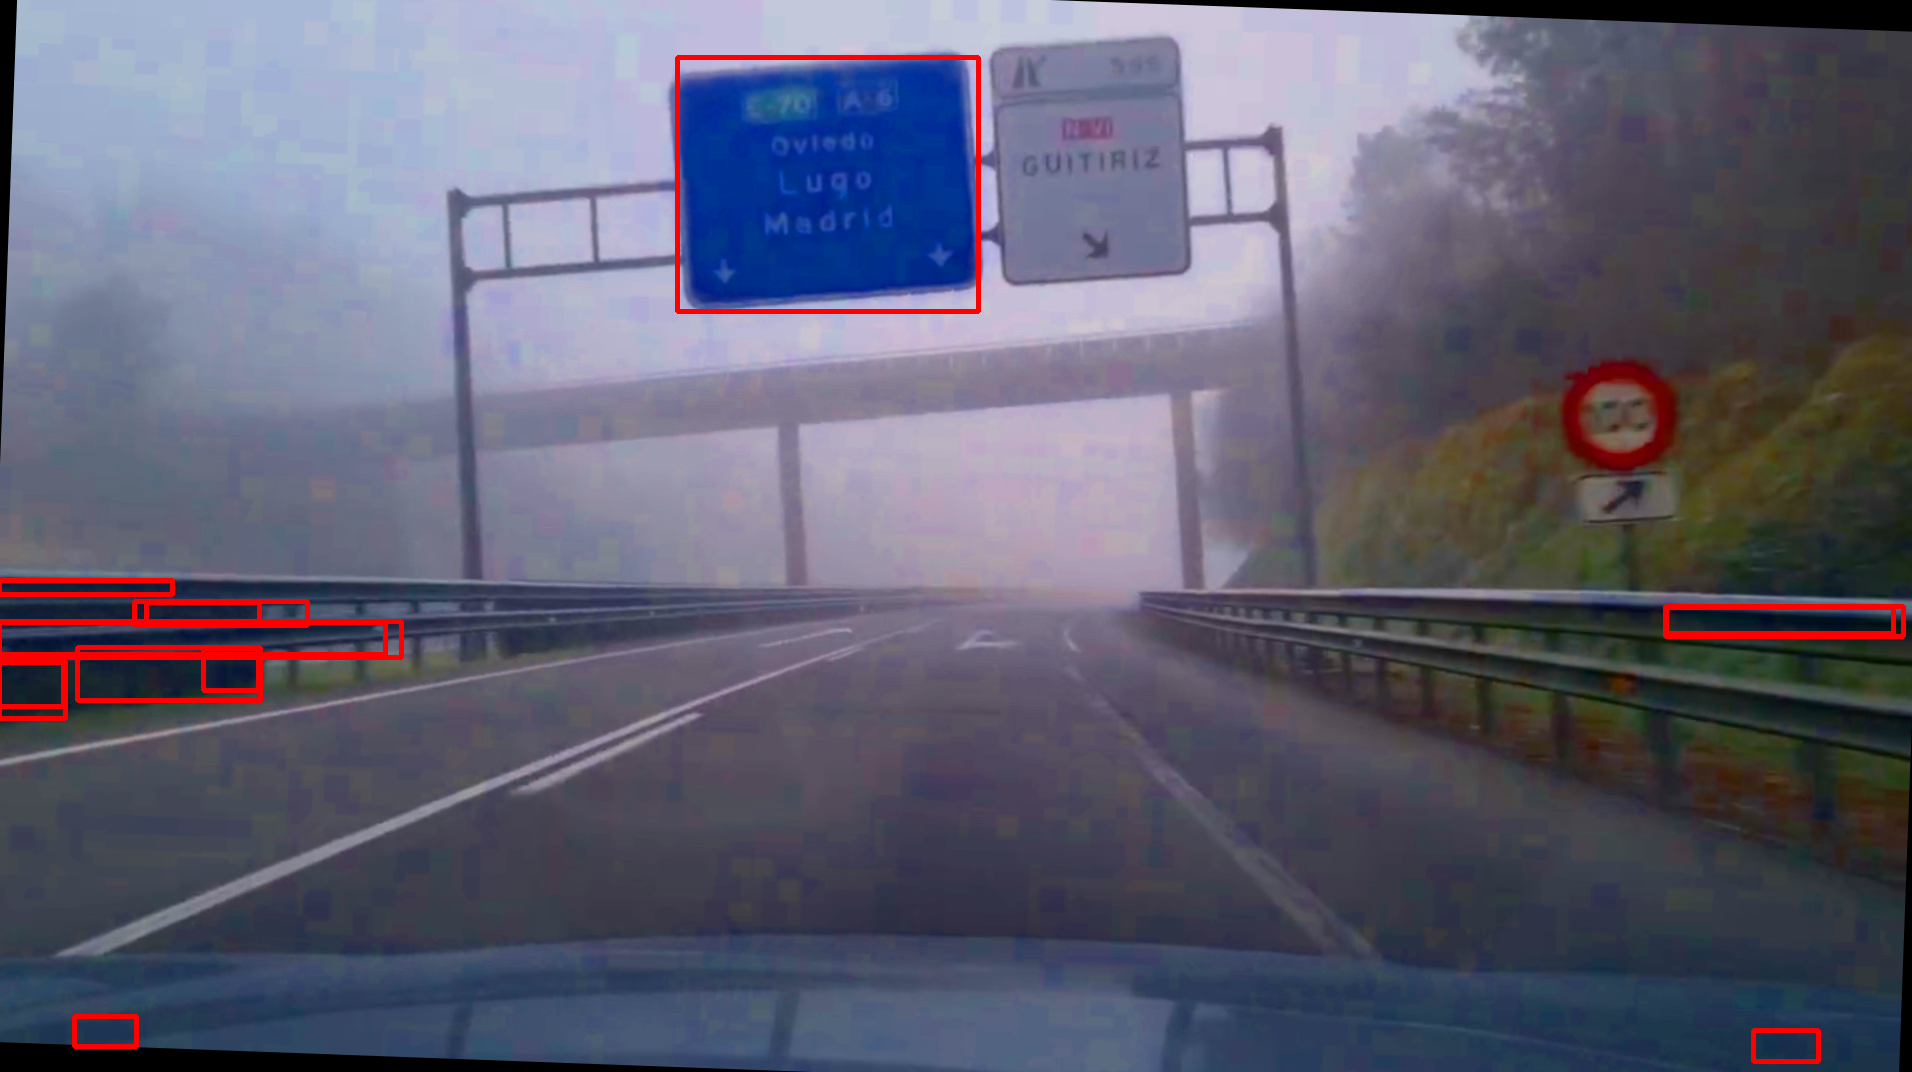
\includegraphics[width=0.6\linewidth]{img/Rectangulos}
	\label{fig:Rectangulos}
\end{figure}

\subsubsection{Filtrar rectángulos por relación de aspecto}
En este apartado se pide que filtremos los rectángulos de las regiones, que hemos dibujado en el paso anterior, por su relación de aspecto con la finalidad de eliminar aquellos que disten mucho de la relación de aspecto de los carteles que se pretenden detectar. 


Además de esto hemos hecho que la función encargada de realizar esto también elimine los rectángulos contenidos dentro de otros. Esto lo hacemos porque queremos solo detectar la región del panel azul, no los subpaneles. La idea es encontrar los subpaneles más adelante, pero solo sobre la imagen del cartel en lugar de hacerlo en la imagen completa, así podemos eliminar detecciones basura que pueda llegar a hacer en la imagen completa, pero de esto ya hablaremos próximamente.


Crearemos dos listas, una para las imágenes con las regiones filtradas dibujadas y otra para las regiones filtradas. 


Luego iteraremos sobre las imágenes, para cada una de estas vamos a crear una lista para guardar las regiones filtradas de esta imagen y copiaremos la imagen para poder dibujar las regiones en la copia así como hemos anteriormente. 


Ahora iteraremos sobre la lista de regiones que pertenecen a esta imagen. Para cada región que hay en la lista vamos a usar \textit{cv2.boundingRect} para obtener el ancho y el alto, con esto podremos calcular la relación de aspecto de las regiones. Nos vamos a quedar con las regiones que tengan una relación de aspecto (ancho/alto) entre 0.6 y 6.5. 


Con la regiones que cumplan esto vamos a hacer la comprobación de si están dentro de otra, en caso de que se cumpla y esté dentro de otra, no nos vamos a quedar con ella, solo queremos quedarnos con las regiones más exteriores con la idea de quedarnos con la región del cartel completo, ya que como hemos dicho antes los subpaneles los buscaremos luego.

Iremos agregando las regiones que cumplan ambas condiciones a la lista \textit{filtered\_regions} y dibujando las mismas en sus imágenes correspondientes, estas las añadiremos también a \textit{images\_filtered\_rectangles}.

Finalmente mostraremos la primera ya la última imagen ya que en estas vemos como se eliminan algunas regiones que no cumplen con las exigencias que queremos. Por último vamos a devolver la lista de imágenes y de regiones filtradas.

Al igual que en los pasos anteriores tenemos una celda comentada para poder ver el resultado en el resto de imágenes. 

Podemos ver el resultado sobre la \textbf{\hyperref[fig:Rectangulos]{Fig. 8}} anterior y la \textbf{\hyperref[fig:RectangulosFiltrados]{Fig. 9}} que tenemos a continuación.
\begin{figure}[h]
	\centering
	\caption{Imagen tras filtrar los rectángulos del paso anterior.}\vspace{0.5cm}
	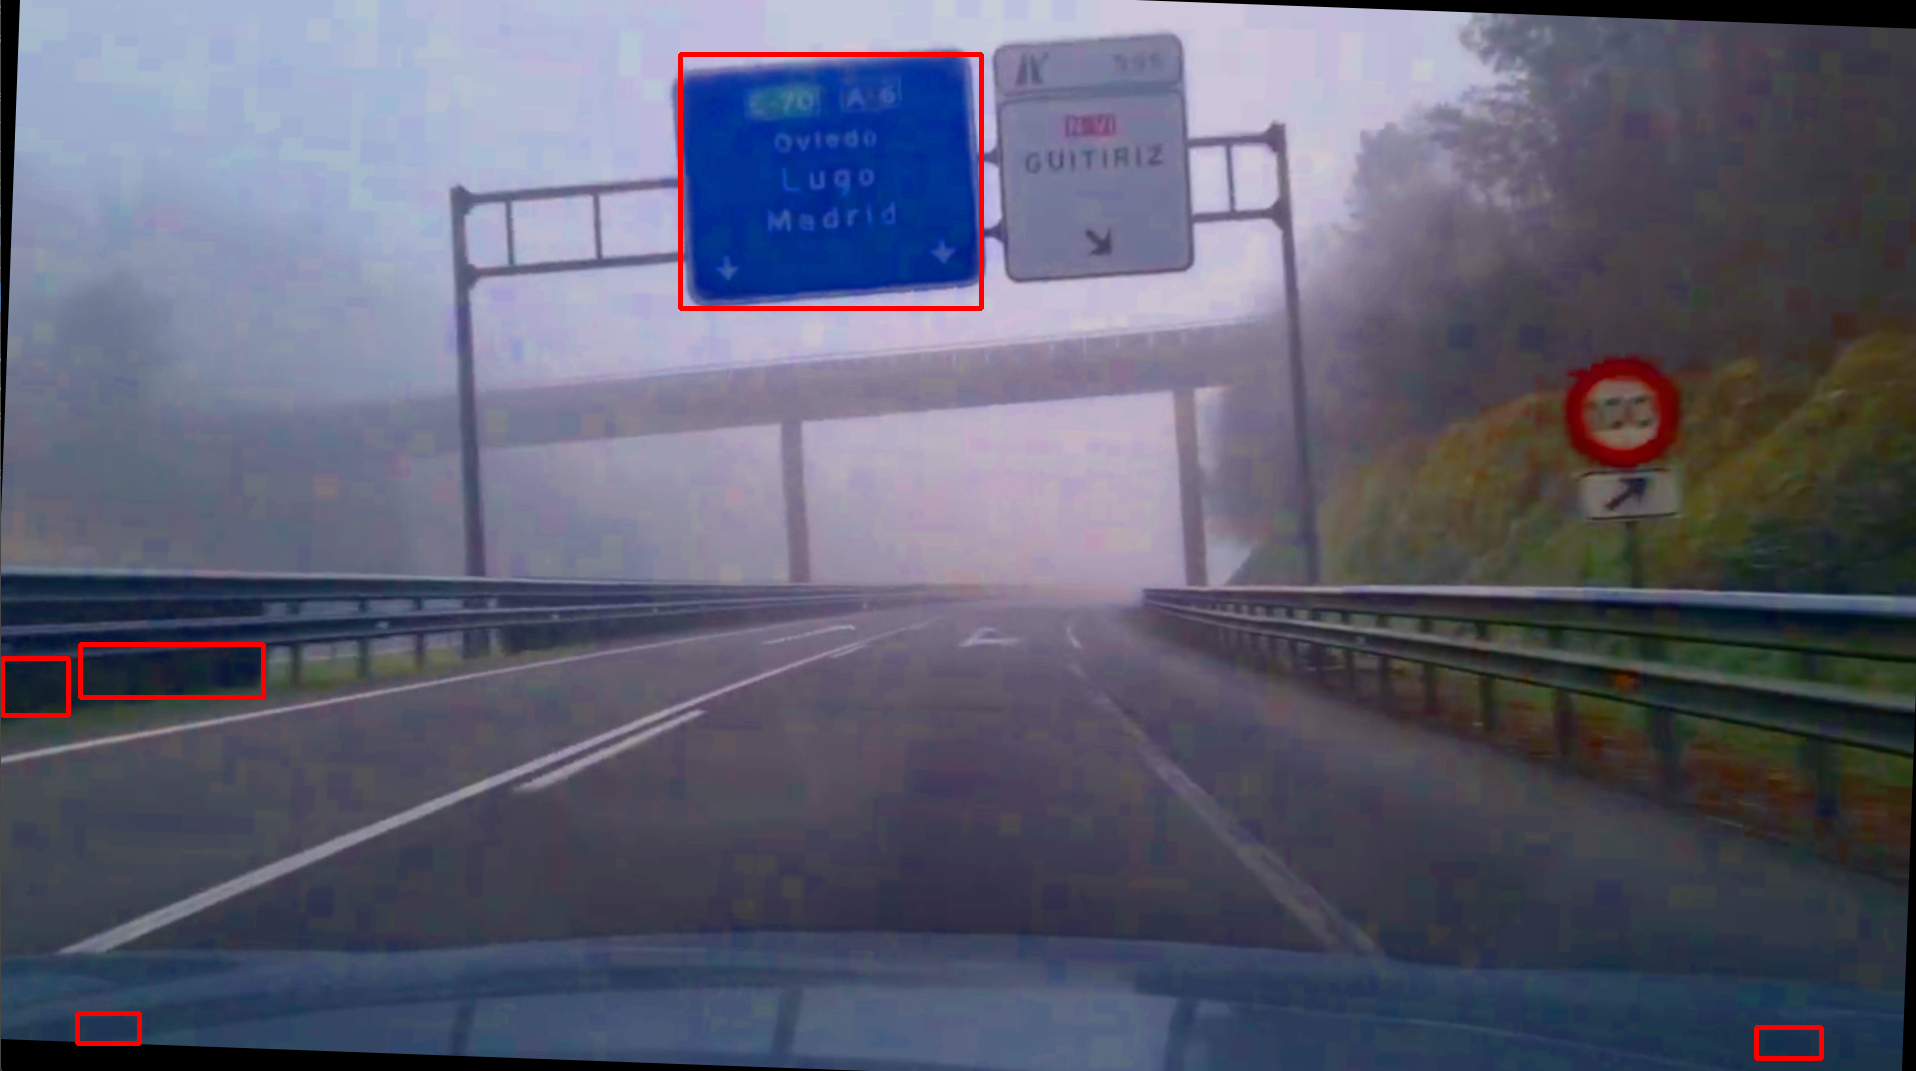
\includegraphics[width=0.6\linewidth]{img/RectangulosFiltrados}
	\label{fig:RectangulosFiltrados}
\end{figure}


\subsubsection{Expandir regiones filtradas}
Al igual que se explica en el enunciado, es posible que haya regiones, sobre las que hemos dibujado un rectángulo, en las que nos haya quedado parte del cartel fuera del rectángulo y para arreglar este pequeño problema, que puede empeorar los resultados en pasos posteriores, tenemos que aumentar el tamaño del rectángulo.

Para solucionar esto tenemos la función \textit{expand\_regions}. Al igual que las funciones anteriores recibirá dos listas. Una de las imágenes normalizadas y la otra de las regiones filtradas en el paso anterior.

La función irá iterando sobre las imágenes de la lista que recibe como primer argumento. Para cada imagen iterará sobre sus regiones filtradas y hallará el punto superior izquierdo (valores \textit{x} e \textit{y}), el ancho y el alto de la región. Una vez tiene estos valores en el caso de los valores de x e y restaremos un valor para que se muevan más hacia arriba a la izquierda. En el caso de la altura y anchura sumaremos un valor porque queremos que sean más grandes. 

Dibujaremos el rectángulo de nuevas dimensiones sobre la copia de la imagen normalizada que hemos hecho previamente. Después de eso vamos crear una pequeña imagen de la región, llamada \textit{pixels\_region}. 
También vamos a guardar en una lista de posibles paneles (\textit{possible\_panels\_img}) este recorte de la imagen normalizada en la que podría haber un panel. Además guardaremos en forma de tupla las coordenadas de cada región ampliada para usarlas más adelante. 

Al igual que hemos hecho en los pasos anteriores vamos a mostrar el resultado de la primera y última imagen y se devolverá la lista de imágenes con las regiones ampliadas dibujadas, otra lista para las coordenadas nuevas de las regiones y la lista de posibles subpaneles. 

Al igual que en los apartados anteriores podemos ver el resultado del resto de imágenes al ejecutar la celda de código siguiente. 

Un ejemplo sería el que podemos ver en la \textbf{\hyperref[fig:RectangulosFiltradosExtendidos]{Fig. 10}}

\begin{figure}[h]
	\centering
	\caption{Imagen tras ampliar los rectángulos del paso anterior.}\vspace{0.5cm}
	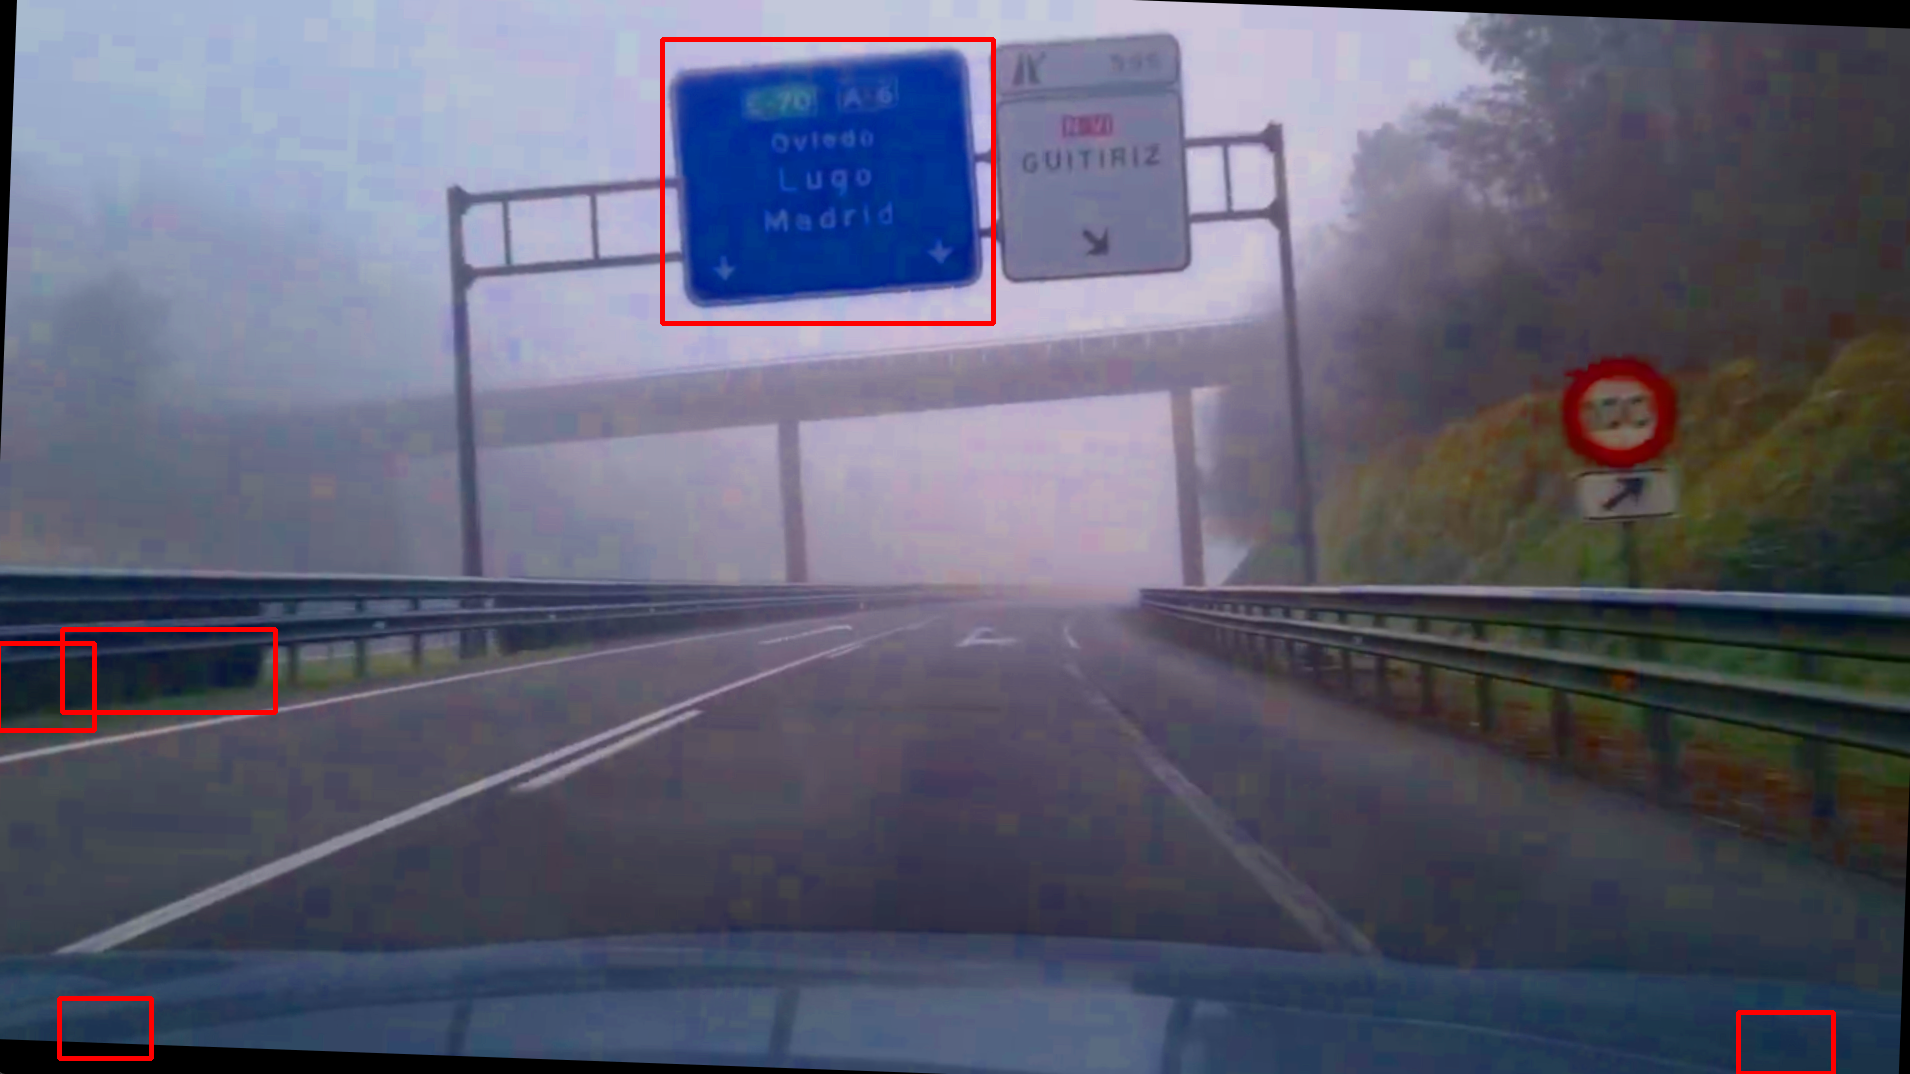
\includegraphics[width=0.6\linewidth]{img/RectangulosFiltradosExtendidos}
	\label{fig:RectangulosFiltradosExtendidos}
\end{figure}


\subsubsection{Detección de subpaneles dentro de la región del cartel}
El proceso de filtrado de las regiones detectadas tenía como objetivo llegar a este punto. Según el enunciado de la práctica, esta parte no se pedía. Nuestra idea era trabajar solo con las regiones que podrían ser carteles a la hora de buscar los subpaneles, ya que pensamos que al haber menos elementos en la imagen seríamos capaces de localizar los paneles de manera más efectiva.

Dentro de este apartado vamos a volver a ejecutar acciones parecidas a las que hemos usado ya, pero en este caso lo haremos sobre los recortes de las imágenes que hemos determinado que pueden ser carteles. 

En la función \textit{detect\_subpanels} vamos a recibir las imágenes normalizadas y la lista de los recortes de cada imagen. Lo que haremos será, imagen por imagen, volver a usar \textit{mser} para detectar las regiones de los subpaneles. Estas imágenes las vamos a redimensionar con \textit{cv2.resize} para hacerlas más grandes. Les aplicaremos en filtro de azul para binarizarlas y usaremos \textit{cv2.Canny} para hallar la imagen de bordes. La dilataremos para no perder detalles en los bordes y aplicaremos \textit{mser} para detectar los subpaneles. Posteriormente a detectar las regiones vamos a ampliarlas y guardar sus coordenadas. 

Finalmente la función va a devolver una lista de recortes de cada región detectada anteriormente, es decir las subregiones dentro de las regiones previas. Estos recortes son posibles subpaneles de las imágenes (\textit{possible\_subpanels}). También vamos a devolver las coordenadas de estas subregiones en la lista 
\textit{subpanel\_coords}.

En la \textbf{\hyperref[fig:subregioness]{Fig. 11}} podemos ver las subregiones detectadas en este paso en la imagen 6.

\begin{figure}[h]
	\centering
	\caption{Subpaneles detectados en la imagen 6.}\vspace{0.5cm}
	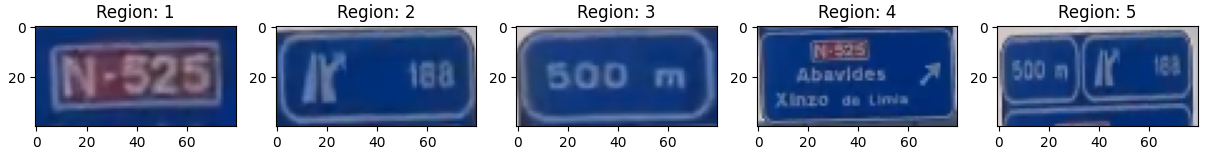
\includegraphics[width=0.6\linewidth]{img/subregiones}
	\label{fig:subregioness}
\end{figure}

\subsubsection{Coordenadas de los subpaneles en la imagen original}
Este es el último paso antes de pasar a la correlación de mascaras. En este paso vamos a corregir las coordenadas que acabamos de obtener de los subpaneles. Esto lo hacemos porque al aumentar el tamaño de la región sobre la que hemos detectado las subregiones, las coordenadas de la subregión también se ven afectadas por el cambio. Para ello tenemos que corregir las coordenadas en el sentido inverso en el que habíamos aumentado la imagen. En el paso anterior hemos multiplicado por tres el ancho y el alto de la imagen y ahora tendremos que dividir por tres. 

Para esto tenemos la función \textit{fix\_coords} de manera similar a como lo hemos ido haciendo anteriormente obtendremos las coordenadas de cada posible subpanel detectado en cada una de las imágenes. Una vez tenemos las coordenadas las ajustamos y las volvemos a guardar en una lista que vamos a devolver. 



\subsection{Correlación por máscaras}
\subsubsection{Mascara ideal}

\begin{figure}[h]
	\centering
	\caption{Panel ideal.}\vspace{0.5cm}
	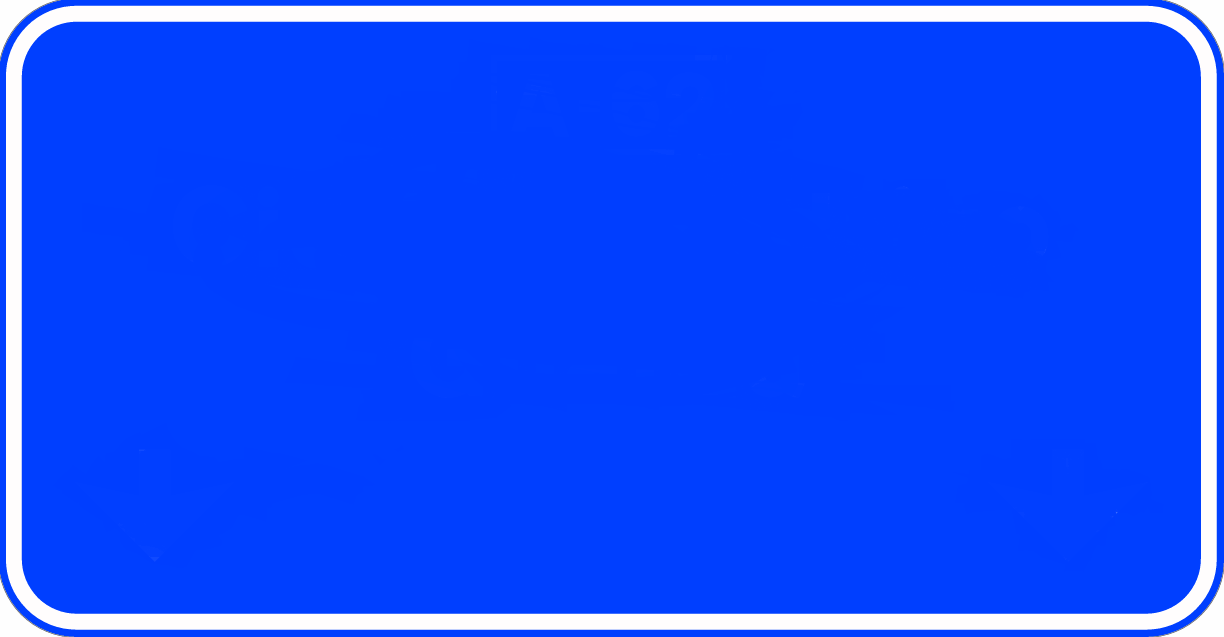
\includegraphics[width=0.4\linewidth]{img/ideal_mask}
	\label{fig:idealmask}
\end{figure}

Para la correcta comprobación de que si una imagen ya filtrada por color es un panel deseado, necesitamos un panel de referencia, para poder indicar como debería ser un panel detectado de forma aproximada.


En la  \textbf{\hyperref[fig:idealmask]{Fig. 12}} podemos ver la imagen de la que partimos para realizar esa mascara ideal que utilizaremos posteriormente. Esta imagen inicial se extrae de la Norma 8.1-IC de señalización vertical de carreteras en España \textbf{[1]}.

Para poder crear la matriz de 1's (para azules) y 0's (para no azules) hacemos uso de un filtro de color. Antes de poder hacer uso del filtro de color necesitamos cambiar el formato de la imagen de \textbf{BGR} a \textbf{HSV}. Este cambio es fundamental porque en el espacio de color HSV, el componente Hue permite una separación clara del color azul, independientemente de las variaciones de iluminación y sombra. Esta conversión y filtrado mejoran significativamente el procesamiento y permiten realizar comparaciones directas con un panel de referencia, facilitando la verificación.

\begin{figure}[h]
	\centering
	\caption{Panel ideal redimensionado y filtrado por color.}\vspace{0.5cm}
	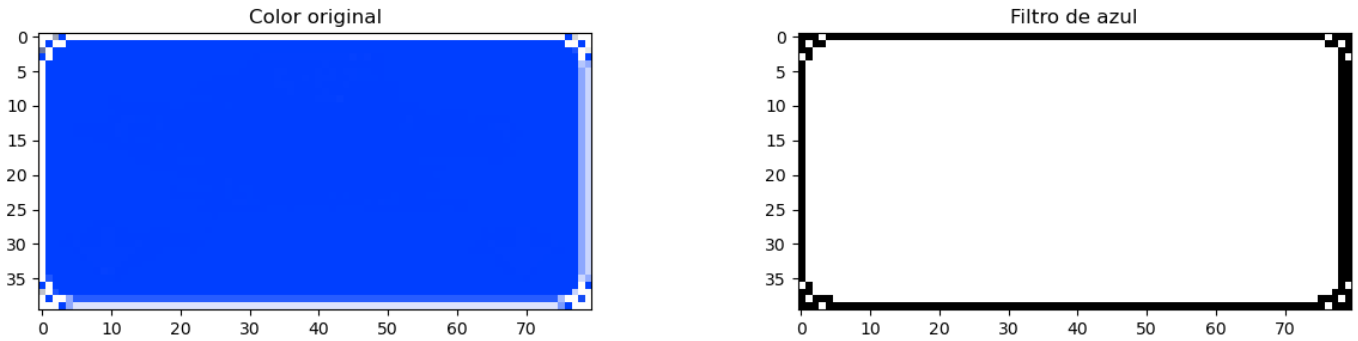
\includegraphics[width=0.9\linewidth]{img/ideal_mask_resized_and_filtered}
	\label{fig:idealmaskresizedandfiltered}
\end{figure}

Ya que nos encontraremos con diferentes paneles de diferentes tamaños, establecemos una tamaño estandar de (80x40) a redimensionar para todos los paneles, tanto detectados como para el ideal. Tras aplicar esta redimensión podemos ya aplicar el filtro de color a nuestro panel, en la \textbf{\hyperref[fig:idealmaskresizedandfiltered]{Fig. 13}} podemos ver el resultado de este proceso con el panel ideal.
\begin{figure}[h]
	\centering
	\caption{Panel detectado redimensionado y filtrado por color.}\vspace{0.5cm}
	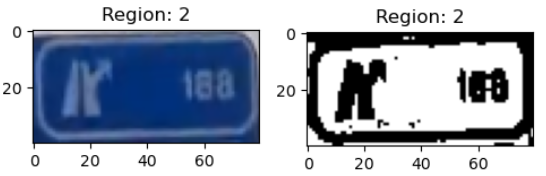
\includegraphics[width=0.7\linewidth]{img/sections}
	\label{fig:sections}
\end{figure}

Respecto a los paneles detectados en la \textbf{\hyperref[fig:sections]{Fig. 14}} podemos ver un ejemplo de su proceso de redimensionado y filtrado por color. De esta manera ya podriamos realizar una comparación y correlación entre detectado/ideal.

\subsubsection{Filtrado por correlación ideal/detectado}
Llegados a este punto quedaría decidir que paneles recibidos son lo suficientemente parecidos al panel ideal. Para ellos realizamos:
\begin{quote}
	\textbf{1.} Una suma de cuantos píxeles azules tiene nuestra máscara ideal. Teniendo en cuenta que es una máscara de 0's y 1's queda bajo la siguiente operación:
	\begin{equation}
		B = \sum_{i = 0}^{39}\sum_{j = 0}^{79} I(i, j)
	\end{equation}
	
	\textbf{2.} Calcular la cantidad de azules que tiene nuestra detección. De igual forma que en el paso anterior:
	\begin{equation}
		B' = \sum_{i = 0}^{39}\sum_{j = 0}^{79} I'(i, j)
	\end{equation}
	\textbf{3.} Calcular un porcentaje de correlación normalizado entre [0,1]. Simplemente haciendo una proporción de $B'$ sobre $B$, en caso de que $B'$ supere a $B$ descartamos esta detección poniendo su proporción a 0. Quedando:
	\begin{equation}
		C = 
		\begin{cases} 
			B'/B & \text{si } B' \leq B, \\
			0 & \text{si } B \leq B'.
		\end{cases}
	\end{equation}
	
	\textbf{4.} Descartamos aquellos valores $C$ que superen un umbral. En este caso se ha puesto uno mínimo de 0'4.
\end{quote}

Posterior a estos pasos nos quedarían las secciones más fiables a la detección deseada, pero nos quedaría eliminar posibles detecciones repetidas.
\subsection{Eliminación de regiones repetidas}
Una vez hemos aplicado todo el proceso del detector y hemos detectado regiones en forma de cuadrados, es posible que tengamos un solapamiento de diversos rectángulos, unos encima de otros. Esto no sería lo óptimo ya que hemos detectado subpaneles, por lo que nunca tendríamos otros subpaneles dentro de estos. Lo mejor sería eliminar los paneles que están dentro de otros y que aporten poco con respecto al rectángulo en el que están contenidos.

El algoritmo escogido es el NMS (Non-Maximum Suppression). Este algoritmo se encarga de eliminar regiones contenidas en otras que tienen una puntuación menor que la que tienen las otras regiones. Se basa en la Intersection over Union (IoU) que se calcula dividiendo la intersección de dos regiones entre la unión entre dos regiones. Podemos ver un ejemplo gráfico en la \textbf{\hyperref[fig:iou]{Fig. 15}}

\begin{figure}[h]
	\centering
	\caption{Cálculo del IoU.}\vspace{0.5cm}
	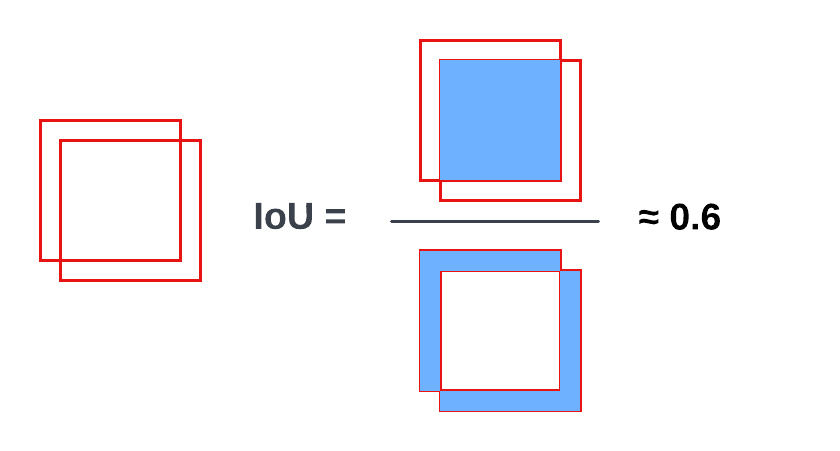
\includegraphics[width=0.5\linewidth]{img/iou.png}
	\label{fig:iou}
\end{figure}

El valor obtenido se encuentra comprendido entre 0 y 1. Un valor de 1 quiere decir que las dos regiones están perfectamente solapadas y un valor de 0 quiere decir que son dos regiones que no se llegan a tocar nunca. 

NMS itera sobre cada uno de los paneles detectados y calcula el IoU sobre esos dos paneles actuales iterados. Si el valor de IoU es mayor que 0 quiere decir que los dos subpaneles están superpuestos. Cuando haya detectado una superposición, entonces se evaluará las puntuaciones de las regiones. Estas puntuaciones las obtenemos en el último paso de la detección a través de la correlación. Escogeremos el panel que tenga mayor puntuación ya que es el panel que mejor se ajusta al panel ideal y eliminamos de la lista la región con menor puntuación. Este proceso se repetirá constantemente con cada uno de los paneles. El pseudocódigo del algoritmo se encuentra representado en la \textbf{\hyperref[fig:nms]{Fig. 16}}
\begin{figure}[h]
	\centering
	\caption{Algoritmo NMS.}\vspace{0.5cm}
	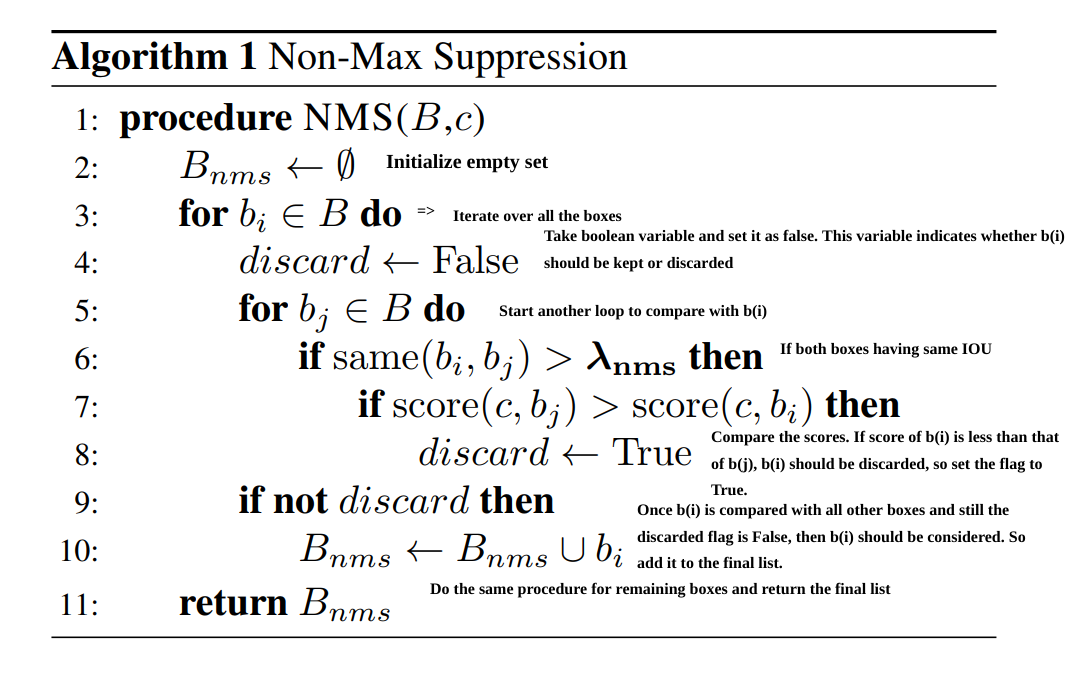
\includegraphics[width=0.7\linewidth]{img/nms.png}
	\label{fig:nms}
\end{figure}

Hemos introducido una pequeña modificación en código para evitar un problema que podíamos tener. El problema en cuestión es que es posible que en algunas ocasiones un panel detectado abarque un poco de región de otro, por lo que el algoritmo lo tomará en cuenta al tener un IoU mayor que 0 y eliminará una región de estas. Esto no es bueno ya que los dos carteles son independientes y no queremos eliminar ninguno de ellos, sino regiones dentro de estos. Para ello, definimos un umbral de IoU de 0.05. Si tenemos un IoU mayor que este umbral significará que tendremos que eliminar una de las regiones ya que es posible que se trate de una región dentro de otra. Así quedaría el algoritmo aplicado en una de las imágenes, como se muestra en la \textbf{\hyperref[fig:nmsAplicado]{Fig. 17}}
\begin{figure}[h]
	\centering
	\caption{Algoritmo NMS aplicado sobre una imagen.}\vspace{0.5cm}
	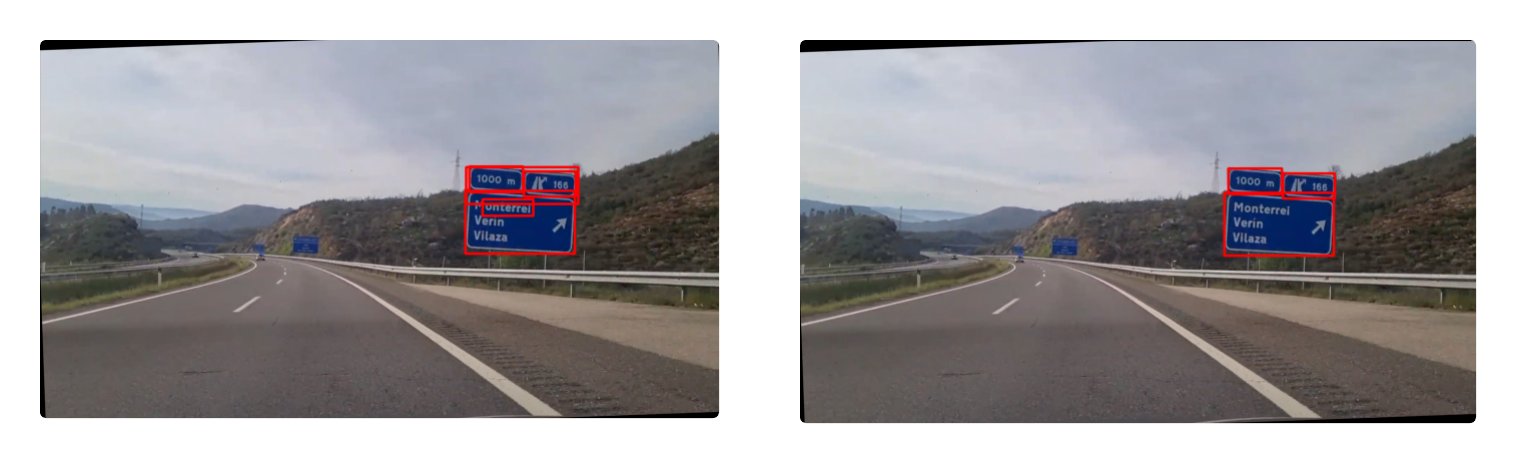
\includegraphics[width=1\linewidth]{img/nmsAplicado.png}
	\label{fig:nmsAplicado}
\end{figure}
\subsection{Validación}
Para finalizar, hemos agregado en una lista las 20 imágenes para nuestro conjunto de prueba. Son imágenes variadas donde hay imágenes con niebla, con más luz, sin carteles o con carteles pequeños, seleccionadas para comprobar la robustez del detector. Para obtener una mejor retroalimentación de la eficacia del detector, hemos anotado manualmente los paneles que realmente aparecen en la escena para luego compararlos con los paneles detectados. Para la anotación de los carteles hemos empleado la página web \href{https://roboflow.com/}{Roboflow} ya que permite anotar regiones de forma manual muy rápidamente. La información anotada se devolverá en un formato JSON donde aparecerán las coordenadas del punto de arriba a la izquierda y el ancho y el alto de cada uno de los rectángulos. El archivo donde se encuentra esta información es el llamado \textit{anotaciones.json}.

Para evaluar la proximidad del cartel detectado con el real usaremos la métrica IoU. Para cada uno de los carteles detectados calcularemos el valor de IoU para cada uno de los carteles reales y nos quedaremos con el valor máximo de este. De este modo cada cartel tendrá su propio valor anotado. Hay que tener en cuenta que este valor puede ser bajo ya que los carteles reales los anotamos en la imagen original, es decir, sin rotarla. Los carteles detectados se encuentran ya en la imagen rotada y por eso el IoU puede resultar bajo. Para finalizar, representaremos los carteles detectados junto con el valor IoU, en la \textbf{\hyperref[fig:cartelIoU]{Fig. 18}}
\begin{figure}[h]
	\centering
	\caption{Cartel detectado con valor de confianza.}\vspace{0.5cm}
	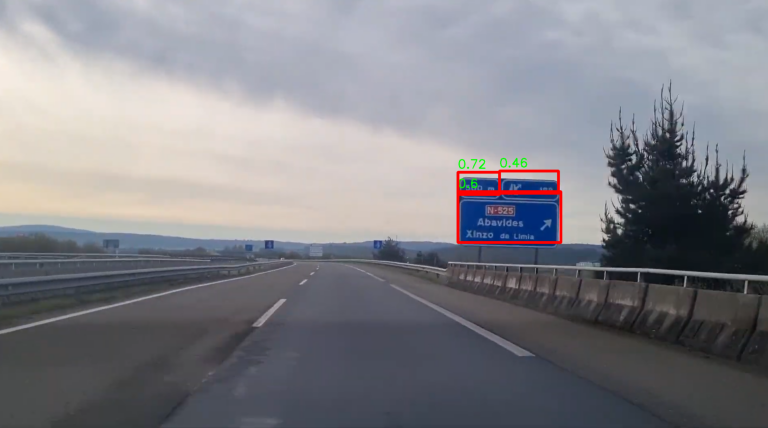
\includegraphics[width=0.7\linewidth]{img/cartelConIoU.png}
	\label{fig:cartelIoU}
\end{figure}



%-------------------------------------------------------
\section{Conclusiones y trabajos futuros}
Como conclusiones después de haber terminado este trabajo podemos decir que lo más complicado ha sido la parte de detectar los carteles con \textit{MSER}, siendo especialmente complicada la tarea, en aquellas imágenes que tenían bastante niebla o que había demasiada luz, haciendo que el color de los carteles fuese más difícil de detectar. 

En la mayoría de los casos de test hemos podido comprobar que los resultados son buenos, incluso en aquellas imágenes en las que había niebla, o que estaban torcidas.

Para mejorar estas detecciones se podría hacer usando un modelo de aprendizaje automático, ya que en general suelen dar mejores resultados que este tipo de algoritmos. 

Por último, comentar que la evaluación a través de IoU ha dado una serie de problemas cuando tenemos paneles dentro de otros paneles ya que el algoritmo implementado no es capaz de generar la lista con los valores correctamente. Aunque hemos pasado por la capa de eliminación de regiones repetidas, tenemos algunos paneles que encapsulan a otros de forma mínima que interfiere en el algoritmo. De las 20 imágenes seleccionadas hay 3 que se le ha dado el valor de 0 a sus paneles para evitar errores mayores.

Agregamos un enlace al repositorio en el que hemos estado trabajando: \href{https://github.com/Im-Lewis/Practica1-VA}{Github}.

%-------------------------------------------------------
\section{Referencias}
[1] \href{https://www.fomento.gob.es/az.bbmf.web/documentacion/pdf/re3723.pdf}{https://www.fomento.gob.es/az.bbmf.web/documentacion/pdf/re3723.pdf}

[2] \href{https://blog.roboflow.com/how-to-code-non-maximum-suppression-nms-in-plain-numpy/}{https://blog.roboflow.com/how-to-code-non-maximum-suppression-nms-in-plain-numpy/}

[3] \href{https://builtin.com/machine-learning/non-maximum-suppression}{https://builtin.com/machine-learning/non-maximum-suppression}

[4] \href{https://roboflow.com/}{https://roboflow.com/}

[5] \href{https://github.com/adheeshc/Traffic-Sign-Recognition/blob/master/README.md}{https://github.com/adheeshc/Traffic-Sign-Recognition/blob/master/README.md}
%-------------------------------------------------------
\end{document}
